\documentclass[a4paper,12pt]{article}
\usepackage[brazil, english]{babel}
\usepackage[utf8]{inputenc}
\usepackage[T1]{fontenc}
\usepackage{geometry}
\usepackage{setspace}
\usepackage{titlesec}
\usepackage{hyperref}
\usepackage{graphicx}
\usepackage{caption}
\usepackage{subcaption}
\usepackage{fancyhdr}

%%%%%%%%%%%%%%%%%%%%%%%%%%%%%%%%%%%%%%%%%%%%%%%%%%
% These are some new commands that may be useful 
% for paper writing in general. If other new commands
% are needed for your specific paper, please feel 
% free to add here. 
%
% The currently available commands are organized in: 
% 1) Systems
% 2) Quantities
% 3) Energies and units
% 4) particle species
% 5) Colors package
% 6) hyperlink
%%%%%%%%%%%%%%%%%%%%%%%%%%%%%%%%%%%%%%%%%%%%%%%%%%

\usepackage{amsmath}
\usepackage{amssymb}
\usepackage{upgreek}
\usepackage{multirow}
\usepackage{setspace}% http://ctan.org/pkg/setspace
\usepackage{fancyhdr}
\usepackage{datetime}

% 1) SYSTEMS
\newcommand{\btc}               {\textbf{BTC}}
\newcommand{\btcspace}          {\textbf{BTC} }
\newcommand{\pow}               {\textbf{PoW}}

% 4) definition to references, biblatex and hyperlink
\usepackage[backend=bibtex, 
style=nature,  %style reference.
sorting=none,
firstinits=true %first name abbreviate
]{biblatex}

\usepackage{hyperref}
\hypersetup{
    colorlinks=true, %set "true" if you want colored links
    linktoc=all,     %set to "all" if you want both sections and subsections linked
    linkcolor=blue,  %choose some color if you want links to stand out
    citecolor= blue, % color of \cite{} in the text.
    urlcolor  = blue, % color of the link for the paper in references.
}

% 5) Tikz and figures
\usepackage{epsfig}
\usepackage{lmodern}
\usepackage{mathtools}
\usepackage[utf8]{luainputenc}
\usepackage{xspace}
\usepackage{tikz}
\usepackage{pgfplots}
\pgfplotsset{compat=newest}

\usetikzlibrary{positioning}
\usepackage{subcaption}

% 6) colors:
\usepackage{xcolor}
\definecolor{ao(english)}{rgb}{0.0, 0.5, 0.0} % dark green

% 7) Add lines numbers
%\usepackage{lineno}

% add pdf file to thesis:
\usepackage{pdfpages}

\hypersetup{
    colorlinks=true,% make the links colored
    linkcolor=blue
}

\usepackage{setspace}
\addbibresource{bibliography.bib}

\newcommand{\printingbibliography}{%

    \pagestyle{myheadings}
    \markright{}
    \sloppy
    \printbibliography[heading=bibintoc, % add to table of contents
                   title=Refer\^encias % Chapter name
                  ]
    \fussy%
}
\PassOptionsToPackage{table}{xcolor}

\pagestyle{fancy}
\fancyhf{}
\renewcommand{\headrulewidth}{0pt}
\fancyhead[R]{\thepage}

\geometry{a4paper,top=30mm,bottom=20mm,left=30mm,right=20mm}

\titleformat*{\section}{\bfseries\large}
\titleformat*{\subsection}{\bfseries\normalsize}

\title{ \textbf{\large Monitoramento e Análise das Métricas da Blockchain do BTC}}
\author{ANDRÉ VIEIRA DA SILVA}
\date{\today}

\begin{document}

\maketitle

\selectlanguage{brazil}

\begin{abstract}
\textbf{PALAVRAS CHAVE: }.
\end{abstract}

\selectlanguage{english}
\begin{abstract}

\textbf{KEYWORDS: A}.
\end{abstract}

\selectlanguage{brazil}

\newpage
%\hypersetup{linkcolor=blue}
\tableofcontents
\newpage

\setstretch{1.3} % Altere o valor 1.2 para o valor desejado

\section{Introdução}
\hspace{0.5cm}Ao usar a blockchain do Bitcoin (\btc) \cite{nakamoto2008bitcoin}, uma rede descentralizada, 
é possível fazer transações financeiras sem a presença de intermediários. 
As métricas da blockchain, que são dados brutos da blockchain extraídos de 
APIs\footnote{A interface de programação de aplicações, ou API, é a sigla em inglês para interface 
de programação de aplicações. As interfaces de programação de aplicativos (APIs) são uma coleção de ferramentas, protocolos e definições que são usadas para criar aplicações de software.
} que mostram as atividades da blockchain, são usadas para monitorar e 
analisar as métricas da blockchain do \btc.

Na avaliação de criptomoedas e blockchain, as quatro principais métricas são 
a taxa de hash, os endereços ativos, os valores de transação e as taxas.
A taxa de hash de uma blockchain é o poder computacional que os mineradores 
de criptomoedas usam para fazer cálculos em uma blockchain de Prova de Trabalho (\pow)
para criar novos blocos, ou minerar novos tokens. Em outras palavras, é a taxa 
de hash de uma blockchain.

A análise on-chain também inclui observar os movimentos da blockchain e dos usuários 
para obter informações, insights e indicadores sobre o preço de um criptoativo. 
Por exemplo, o \btc: Balanced Price, fornecido pela Glassnode, ``representa a diferença 
entre o preço realizado e o preço transferido" do \btc. 

O indicador fornece o valor nominal do btc e serve como uma guia para saber se o ativo 
está próximo ou não do seu ``valor justo". A dominância do \btc, que calcula a proporção 
total de \btcspace em relação ao mercado de criptoativos, é outro indicador útil.

A métrica pode ser encontrada dividindo o valor da capitalização do \btcspace pela capitalização 
total das criptomoedas mais valiosas e multiplicando por 100.
Um estudo recente realizado pelo MIT Sloan revelou que a realidade da rede \btcspace difere do modelo 
idealizado e descentralizado que os entusiastas de criptomoedas costumam apresentar. O estudo 
mostrou que grandes jogadores concentrados ainda dominam a rede e que an estrutura dos principais 
participantes é diferente do que se pensava.

Em resumo, a análise das métricas da blockchain do \btcspace é uma ferramenta útil para entender 
o comportamento da rede e dos usuários, bem como para avaliar o valor do \btcspace e outras criptomoedas. 
Para investidores e entusiastas de criptomoedas, as métricas de blockchain e an análise de blockchain 
de podem fornecer informações úteis. Nas pr\'oximas se\c{c}\~oes ser\~ao descritos os termos t\'ecnicos
sobre blockchain.

\section{O que \'e an\'alise on-chain?}
\hspace{0.5cm}A an\'alise on-chain é um método para examinar dados e extrair \textit{insights} 
sobre as dados da blockchain, que é a tecnologia que sustenta o \btc. Em outras palavras, a blockchain 
é a livro cont\'abil p\'ublico onde as transações são registradas em uma database imut\'avel. 
Utilizando m\'etricas on-chain, esta base de dados é utilizada para avaliar o sentimento do mercado 
de criptomoedas.

A alteração da informação após a inclusão de um bloco na blockchain é extremamente difícil, 
se não impossível. Al\'em disso, os dados da blockchain são armazenados de forma distribu\'ida 
entre os participantes da rede, em vez de em um único local. Isso o distingue de uma database convencional. 
A explosão de novos tipos de negócios e serviços financeiros que antes não eram possíveis foi desencadeada 
por esse conceito fundamental de permitir a transferência e armazenamento de transactions de um local 
para outro.

As m\'etricas on-chain que são construídas a partir da dados da blockchain, oferecem uma visão 
abrangente da rede do \btc. As principais métricas on-chain são citadas abaixo:

\begin{itemize}
    \item As entradas e saídas de \btcspace das exchanges\footnote{O mercado de criptomoedas é um espaço 
    onde as pessoas podem comprar e vender diferentes tipos de moedas digitais, como Bitcoin, 
    Ethereum e muitas outras. O termo ``exchange'' refere-se a uma plataforma online que permite 
    que os indivíduos negociem essas criptomoedas entre si.}, 
    \item Carteiras ativas de \btc, 
    \item Balan\c{c}o de \btcspace nas carteiras das Baleias,
    \item A dificuldade para minerar um bloco,
    \item Valor da recompensa para os mineradores em 24 horas,
    \item A oferta de \btcspace pode ser dividida em duas categorias principais: líquida e ilíquida.
\end{itemize}

Os mais populares provedores de dados on-chain, como o Glassnode\footnote{https://glassnode.com/} e 
Coin Metrics\footnote{https://coinmetrics.io/}, oferecem 
muitas outras m\'etricas. O objetivo principal da an\'alise on-chain é examinar 
os dados s\~ao como um term\^ometro da rede \btcspace e do mercado, para determinar as tendências 
de preços do \btcspace atual e futuro usando métricas.

\subsection{Os fundamentos da Blockchain}

\hspace{0.5cm}Para entender como funciona a tecnologia blockchain, você deve aprender as bases. 
Estas são as principais noções:

\begin{enumerate}
    \item \textbf{Blocos}: Uma blockchain é uma estrutura de dados composta por cadeia de blocos. 
    Cada bloco é composto por um conjunto de informações ou transações. Uma cadeia contínua é 
    criada quando os blocos são conectados de forma cronológica.

    \item \textbf{Transações}: As transações são ações ou eventos que estão registrados na blockchain. Por exemplo, 
    transferir bitcoins de um indivíduo para outro pode ser uma transação em uma blockchain de criptomoeda.
    
    \item \textbf{Criptografia}: técnicas de criptografia são usadas na blockchain para garantir a segurança dos dados. 
    Os algoritmos criptográficos protegem as transações e as informações em um bloco, tornando-as 
    extremamente difíceis de alterar.

    \item \textbf{Rede descentralizada}: A blockchain é distribuída em uma rede de computadores, também conhecidos 
    como ``nós'', que são envolvidos na validação e armazenamento dos blocos. A rede não tem uma autoridade 
    central; em vez disso, a comunidade local o administra.

    \item \textbf{Consenso}: O processo pelo qual os nós da rede concordam sobre a validade das transações e 
    como elas devem ser adicionadas à blockchain é conhecido como consenso. Os algoritmos de consenso 
    Prova de trabalho (PoW) e 'Proof of Stake' (PoS) são usados em várias blockchains.

    \item \textbf{Imutabilidade}: Uma transação é praticamente imutável quando é registrada em um bloco e 
    adicionada à blockchain. Isso indica que alterar ou apagar uma transação após sua inclusão 
    na blockchain é extremamente difícil ou impossível.

    \item \textbf{Contratos inteligentes}: Algumas blockchains, como an Ethereum, permitem a criação de contratos 
    inteligentes. Esses programas são executáveis por computador e têm a capacidade de automatizar a
     execução de contratos e acordos, eliminando a necessidade de intermediários.

     \item \textbf{Chave pública e privada}: Duas chaves são usadas nas carteiras de criptomoeda: uma para 
     receber fundos e outra para autorizar transações. Como permite que o proprietário use o dinheiro associado 
     à chave pública, a chave privada deve ser mantida em segredo.

     \item \textbf{Mineração (em PoW)}: Os mineradores usam poder computacional em blockchains PoW, 
     como o Bitcoin, para resolver problemas matemáticos difíceis e adicionar novos blocos à blockchain. 
     Eles recebem criptomoedas como recompensa por seu trabalho.

     \item \textbf{Armazenamento distribuído}: Uma cópia completa da blockchain é armazenada em cada nó da rede blockchain. 
     Isso aumenta a redundância e a segurança da informação.
\end{enumerate}

Essas são as bases da tecnologia blockchain. Ela inclui aplicativos que vão além das criptomoedas, como 
contratos inteligentes e muito mais, oferecendo uma maneira transparente, segura e descentralizada de registrar 
transações e informações. A blockchain é a tecnologia fundamental por trás da criptomoeda \btc. 


\subsection{Bitcoin: Um Sistema de Dinheiro Eletrônico}

\note{Em 2008, um indivíduo ou grupo com o pseudônimo Satoshi Nakamoto sugeriu um sistema de pagamentos 
decentralizado para pessoas com outras pessoas. O principal obstáculo para digital payments é evitar 
que os mesmos bens sejam gastos dois vezes. De acordo com o bitcoin 'white paper', uma nova abordagem 
para validar transações por meio de criptografia resolve o problema conhecido como 'gasto duplo'. 
Esses e outros avanços para a tecnologia de um livro cont\'abil distribu\'ido constitui a base para 
ativos digitais.}

\subsection{História do Bitcoin e a importância de Satoshi Nakamoto}

\hspace{0.5cm}O artigo ``Bitcoin: A Peer-to-Peer Electronic Cash System'' foi o primeiro whitepaper 
que apresentou o Bitcoin. Foi publicado em outubro de 2008. Satoshi Nakamoto escreveu um whitepaper 
que apresentava uma ideia revolucionária de uma moeda digital que funcionaria em uma rede descentralizada,
eliminando a necessidade de intermediários financeiros como bancos.

\subsection{Blockchain: O Livro-Razão Público do Bitcoin}

\hspace{0.5cm}O fundamento sobre o qual o Bitcoin e muitas outras criptomoedas são construídas 
é o blockchain, que significa ``cadeia de blocos'' em português. Ele funciona como um registro 
público e descentralizado de todas as transações que ocorrem em uma rede de criptomoeda. 
O papel do blockchain no Bitcoin é essencial para garantir a segurança, transparência e 
integridade da rede.

\subsubsection{Arquitetura da Blockchain}
\hspace{0.5cm}O blockchain é chamado de ``cadeia de blocos'' porque é composto por um conjunto 
de blocos que estão conectados de forma cronológica. Cada bloco contém um conjunto de transações que 
os mineradores da rede validaram. Aproximadamente a cada dez minutos, essas transações são organizadas 
em blocos.

\textbf{Principais componentes de um bloco}: 

\begin{enumerate}
\item \textbf{O cabeçalho do bloco}: Contém informações importantes como o número do bloco, 
um registro da data e hora, um hash que identifica o bloco anterior (exceto no primeiro bloco, conhecido como 
``bloco gênesis'') e um hash que representa o conteúdo do bloco atual.

\item \textbf{Transações}: Um conjunto de transações que detalham como transferir bitcoins de um 
endereço para outro é exibido em cada bloco. Para garantir a segurança e an autenticidade dessas 
transações, elas são criptografadas e assinadas digitalmente.
\end{enumerate}

O blockchain do Bitcoin funciona em uma rede mundial de computadores descentralizados que 
trabalham em conjunto para validar e registrar essas transações. A ``mineração'' é o processo 
de validar e adicionar um novo bloco à cadeia.

\textbf{Mineração e Consenso}: 

\begin{itemize}
\item Mineradores de Bitcoin lutam para resolver quebra-cabeças matemáticos complicados conhecidos como 
``prova de trabalho''. O direito de adicionar um novo bloco ao blockchain pertence ao minerador que é o 
primeiro a resolver o quebra-cabeça.

\item Os outros nós da rede verificam e aceitam as transações em um bloco a cada vez que é adicionado. 
Isso os leva a concordar sobre o estado atual do blockchain.
\end{itemize}

\subsubsection{Segurança e Integridade}
\hspace{0.5cm}O blockchain do \btcspace é altamente seguro e resistente a manipulações devido a várias 
características:

\begin{itemize}
\item \textbf{Criptografia}: As transações no blockchain são protegidas por algoritmos criptográficos 
robustos.

\item \textbf{Descentralização}: A rede é distribuída globalmente, tornando difícil para qualquer entidade 
controlar a maioria dos nós.

\item \textbf{Imutabilidade}: Uma vez que um bloco é adicionado ao blockchain, é extremamente difícil 
(quase impossível) alterá-lo sem o consenso da maioria da rede.

\end{itemize}

\subsubsection{Trilema das Blockchains}
\hspace{0.5cm}O ``trilema das blockchains'' no contexto do Bitcoin (\btc) refere-se aos três desafios fundamentais 
que a rede Bitcoin enfrenta ao tentar equilibrar três características principais: 

\important{
    \begin{itemize}
    \item \textbf{Segurança}, (Segurity)
    \item \textbf{Descentralização}, (Decentralization)
    \item \textbf{Escalabilidade}. (Scalability)
    \end{itemize}
    }

\begin{itemize}
    \item \textbf{Segurança}: A segurança do \btcspace deve ser priorizada. Isso significa que todos os 
    dados e transações que estão no blockchain do Bitcoin devem ser inalteráveis e indetectáveis. 
    As informações no blockchain não podem ser comprometidas por meio da criptografia e do protocolo 
    de consenso à prova de trabalho.

    \item \textbf{Descentralização}: A descentralização é um pilar do \btc. Isso significa que, 
    em vez de ser controlado por uma única entidade ou grupo, a rede deve ser operada e mantida 
    por uma ampla rede de nós descentralizados. Isso fortalece a resistência à censura. Além disso, 
    evita um único ponto de falha.

    \item \textbf{Escalabilidade}: A capacidade do \btcspace de lidar com uma quantidade significativa 
    de transações sem comprometer sua descentralização e segurança é chamada de escalabilidade. Isso é 
    essencial para atender à crescente demanda por transações e garantir que o Bitcoin seja uma moeda 
    viável em larga escala.

\end{itemize}

Esses desafios são frequentemente descritos como um ``trilema'' porque é difícil atender 
completamente a todos eles simultaneamente na rede \btc. Aqui estão os componentes do 
trilema específicos para o \btc.

\begin{figure}[!h]
    \centering
    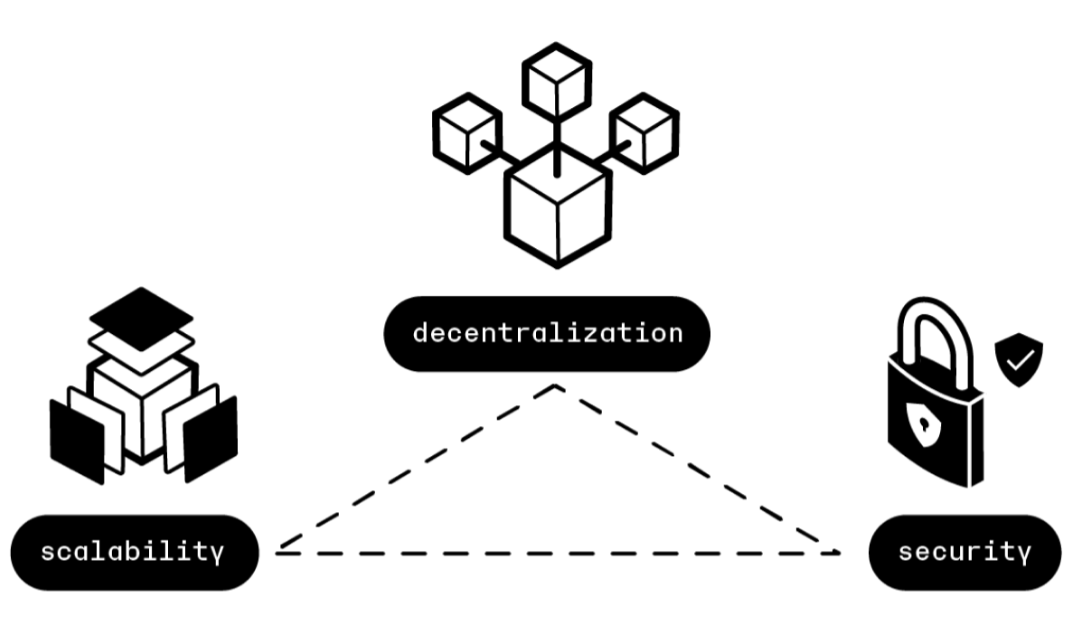
\includegraphics[width=0.8\textwidth]{images/trillemabtc.png}
    \caption{Trillema das Blockchains. Figura retirada do site \href{https://coinloan.io/blog/what-is-blockchain-trilemma/}{What is Blockchain Trillema}.}
    \label{trillemablockchain}
\end{figure}

O problema com o trilema do \btcspace é que muitas vezes há um compromisso nos outros dois 
ao tentar melhorar um. Por exemplo, aumentar a escalabilidade pode exigir uma implementação 
de soluções de segunda camada, como a Lightning Network, que têm o potencial de impactar a
descentralização. De forma semelhante, o foco na segurança máxima pode afetar a escalabilidade.

A evolução e o crescimento do \btcspace envolveram a busca de soluções para o trilema. 
Para equilibrar melhor os três fatores, podem ser incluídos atualizações de protocolo, 
otimizações de software, ajustes nas configurações e soluções de segunda camada. Manter o \btcspace seguro, 
descentralizado e escalável é um objetivo que os desenvolvedores e a comunidade estão continuamente 
trabalhando para resolver. É fundamental entender que o trilema é uma questão complicada e flutuante 
no desenvolvimento do \btc, e encontrar a maneira de equilibrar adequadamente esses três aspectos é 
fundamental para seu sucesso contínuo.

\section{As Principais Métricas do Blockchain}




%%%%%%%% Bibliography 
% Os comandos para incluir as referências bibliográficas
\printingbibliography

\end{document}
